\documentclass{article}
% ============= Page size margins etc.
% ============= This offers great flexibility in terms of document size
\usepackage{geometry}
\geometry{twoside,
          letterpaper, % i.e, paperwidth=210mm and paperheight=297mm,
          top=35mm,
          bottom=40mm,
          left=25mm,
          right=25mm,
}
% =========== Math related stuff
% There are more tools for handling fractions etc.
% but can be left out until the need is obvious
\usepackage{mathtools} %<- Fixes, enhances amsmath package (loads amsmath too so no need to load it)
\usepackage{amssymb,amsthm}% Standard AMS tools

% =========== Graphics-related stuff
\usepackage{graphicx} % don't load epsfig or psfig
\usepackage{hyperref}

\usepackage{xcolor}


%Let's replicate the handout for demo, I'll call mytitle
\newcommand{\myTitleBox}{
\noindent\makebox[\linewidth][c]{%
  \colorbox{gray!30}{%
    \parbox{\paperwidth}{%
      \hspace*{\dimexpr\hoffset+\oddsidemargin+1in\relax}%
      \begin{minipage}{\dimexpr\textwidth-2\fboxsep-2\fboxrule\relax}
      {\centering\Large\topicsCovered\par}\vspace{2mm}
      \courseTitle\hfill\sectionTime\\
      \csname @author\endcsname\hfill\authorContact
      \end{minipage}
    }%
  }%
}
}

\setlength{\parskip}{1em}
\setlength{\parindent}{0pt}
% Now let's fill it up

\newcommand{\courseTitle}{APCOMP209a: Introduction to Data Science}
\newcommand{\sectionTime}{Wed/Thurs 2:30-3:30 \& Wed 5:30-6:30}
\newcommand{\topicsCovered}{Linear Models and Linear Regression}
\newcommand{\authorContact}{nhoernle@g.harvard.edu}

\author{Nick Hoernle}


\begin{document}
\myTitleBox

\section{Recap}
Recall that we have an unknown function ($f$) that relates the response variable ($y_i$) to the input vector ($\mathbf{x_i}$). Our goal is to find a model ($\hat{f}$) (i.e. we are approximating $f$) such that a \textit{loss function} is minimised. We may want to use this model for \textbf{prediction} and/or for \textbf{inference}.

We can say we have a training dataset with N \textit{i.i.d} training datapoints $(y_i, \mathbf{x_i})$, $i=1,\dots,N$, which each consist of a one dimensional response variable and a $p$ dimensional input vector ($y_i \in \mathbb{R}$ and $x_i \in \mathbb{R}^p$).

An \textbf{assumption} in linear regression is that the predictor function that we are approximating is linear. We can then write this relationship as:
\begin{align*}
y_i &= f(x_i) = \beta_0 + \sum\limits_{j=1}^{p}x_{ij}\beta_j + \epsilon_i\\
Y &= f(\mathbf{X}) = \mathbf{X} \beta + \mathbf{\epsilon}
\end{align*}

Where $\mathbf{X}$ now refers to an $N\times(p+1)$ dimensional matrix.

For now, let us assume that we know `$p$' in advance (we will deal with this assumption more under the \textbf{model selection} topic in this class). We are now able to construct our \textit{model}:
$$
\hat{Y} = \hat{f}(\mathbf{X}) = \mathbf{X} \hat{\beta}
$$
Recall, that there is a portion of variance in the data that can be explained by the model and there is a portion of the variance in the data that is purely statistical noise and cannot be explained by the model. Heuristically, we aim to minimise some distance metric between our predictions $\hat{Y}$ and the true training data $Y$.

% \noindent\fbox{\begin{minipage}{\dimexpr\textwidth-2\fboxsep-2\fboxrule\relax}
% \textbf{Question Box:}
% \begin{enumerate}
%   \item What does $\epsilon$ represent?
%   \item We referred to a `pre-defined \textit{loss function}', how is this chosen? Can you think of common loss functions and motivate why one might be better than another?
% \end{enumerate}
% \end{minipage}}
% \newpage
For linear regression, we make the \textbf{assumption} that the noise ($\epsilon$) is distributed as a Normal random variable with mean 0, variance $\sigma^2$. I.e. $\epsilon \sim \mathcal{N}(0, \sigma^2)$. You can then follow that $Y \sim \mathcal{N}(\mathbf{X} \beta, \sigma^2)$. It is therefore common to denote the linear regression problem as finding the \textbf{expected value} of $Y$ given the input variables $\mathbf{X}$.

$$
E[Y \vert \mathbf{X}] = \mathbf{X} \hat{\beta}
$$

\textit{More on this topic in upcoming classes.}

\section{Matrix Algebra Recap}
\textit{Please refer to the really useful Matrix Cookbook for a more detailed recap on matrix operations: (\url{http://www2.imm.dtu.dk/pubdb/views/edoc_download.php/3274/pdf/imm3274.pdf})}

We'll be using the following results (although I highly recommend you download a copy of the cookbook \cite{petersen2008matrix} and keep it handy):

\begin{enumerate}
  \item $(AB)^{-1} = B^{-1}A^{-1}$
  \item $(A^T)^{-1} = (A^{-1})^{T}$
  \item $\Vert x \Vert_2^2 = x^Hx$ \dots (note that `H' refers to the Hermitian vector (transposed, complex conjugated) and thus for most of our purposes (i.e. Real domain), the transposed (T) vector is sufficient).
  \item $\frac{\partial}{\partial x}[(b - Ax)^T(b-Ax)] = -2A^T(b-Ax)$
  \item The density of $x \sim \mathcal{N}(\mu, \Sigma)$ is $p(x) = \frac{1}{\sqrt{det(2\pi \Sigma)}}exp[-\frac{1}{2}(x-\mu)^T \Sigma^{-1}(x-\mu)]$
\end{enumerate}

\textit{The above assumes A and B are matrices, x and b are vectors.}

\section{Minimising the Loss Function}
We have a system where the data $Y$ and our model $\hat{Y} (=\mathbf{X}\hat{\beta})$ differ by some \textbf{residual} amounts. Our goal is to find the unknown parameters $\hat{\beta}$ such that the residuals are minimised. Since we are trying to minimise the error of the model over all of the datapoints, it makes sense to minimise a sum of all square magnitudes of errors:
$$
SSE = \sum\limits_{i=0}^{N}\vert residual_i \vert^2 = \sum\limits_{i=0}^{N}\vert y_i - \beta\mathbf{x}_i^T \vert^2 = \Vert Y - \mathbf{X}\hat{\beta} \Vert_2^2
$$

Choosing to minimise the \textit{sum of square errors (SSE)}:
$$
\hat{\beta} = \min_{\hat{\beta}} (SSE) = \min_{\hat{\beta}}\Vert Y - \mathbf{X}\hat{\beta} \Vert_2^2 = \min_{\hat{\beta}}((Y - \mathbf{X}\hat{\beta})^T(Y - \mathbf{X}\hat{\beta}))
$$

Finding the gradient and setting it to zero, we can obtain:
\begin{align*}
\frac{\partial SSE}{\partial \hat{\beta}} &= -2\mathbf{X}^T(Y - \mathbf{X}\hat{\beta}) = 0\\
\mathbf{X}^T\mathbf{X}\hat{\beta} &= \mathbf{X}^TY\\
\hat{\beta} &= (\mathbf{X}^T\mathbf{X})^{-1}\mathbf{X}^TY
\end{align*}

\section{Linear Regression as a Projection}
Our predictions $\hat{Y} = \mathbf{X}\hat{\beta} = \mathbf{X}(\mathbf{X}^T\mathbf{X})^{-1}\mathbf{X}^TY$ can be condensed into the following equation:

$$
\hat{Y} = \mathbf{H}Y
$$

Where $\mathbf{H} = \mathbf{X}(\mathbf{X}^T\mathbf{X})^{-1}\mathbf{X}^T$. This matrix is often referred to as ``the hat matrix as it puts the hat on the y'' \cite{friedman2001elements}. Note that the columns of the $\mathbf{X}$ matrix form a subspace of $\mathbb{R}^N$ that is referred to the column space of $\mathbf{X}$.

\begin{figure}[h]
\center
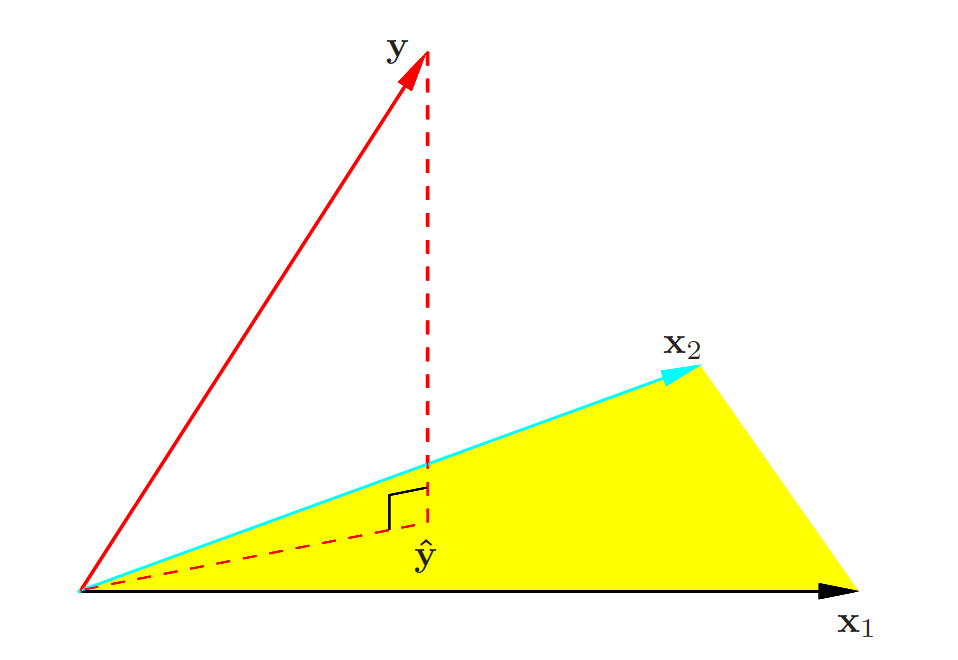
\includegraphics[width=8cm]{l_r_projection}
\caption{Diagram showing the vector $y$ projected onto the subspace spanned by the matrix $\mathbf{X}$ in this case with two linearly independent dimensions\cite{friedman2001elements}}\label{l_r_projection}
\end{figure}

When we minimise the error between the solution $Y$ and the vector projection $\hat{Y}$ (see Figure \ref{l_r_projection}), the result is that the error must be orthogonal to the column space (i.e. the solution to the least squares problem is the orthogonal projection of the vector $Y$ onto the subspace that is spanned by the columns of $\mathbf{X}$). \textit{Why is this useful to know?} It is useful to visualise the prediction vector $\hat{Y}$ as a linear combination of the columns of $\mathbf{X}$ and this $\hat{Y}$ vector is the `closest' in $\mathbb{R}^N$ that the prediction can get to the real solution (try to visualise this in terms of the reducible and irreducible errors discussed in class).

\section{Statistical Inference and Hypothesis Testing}
Remember that our ultimate goal is to model the linear relationship between various predictors and the response variable. If our model is `good', not only can we use it to make \textbf{predictions} about future or unknown events, but we can also use it to make \textbf{inferences} about the underlying structure of the system. Up until now we have assumed that we \textit{knew} the true number of predictors and that we \textit{knew} they had a \textit{linear} relationship with the response variable. This is often not the case and therefore in statistical inference, assumptions of the model have to be validated before any inference is done.

To begin, let us tackle the idea of having a linear relation. Given data $(y_i, \mathbf{x_i})$, $i=1,\dots,N$, we can ask the question: \textit{is there a true linear relationship between the predictor variable $x$ and the response variable $y$?} We need to answer this question with \textit{statistical evidence}. For example, consider the plots below where there are 10 datapoints sampled from four different linear relationships. We need a robust method for analysing which relations are \textit{statistically significant} and which are not (as it is clear that in all cases, due to the noise in the system, there is not one linear function relating the predictor and the response variables). We thus turn to statistical `t-' (\ref{t-test}) and `F-' (\ref{f-test}) tests to make conclusions about the underlying system given the sample of data we have observed.

\begin{figure}[h]
\center
\includegraphics[width=15cm]{hypothesis_testing_ex}
\caption{Example of a linear function with varying amounts of noise. We need a robust way of determining if our samples actually have a relationship or if we are just observing noise.}\label{im:hypothesis_test}
\end{figure}

The idea of hypothesis testing is to make some assumptions about the nature of the true system, given the sample that you are observing, and \textbf{if those assumptions hold}, you can conclude whether or not a certain null hypothesis is probabilistically reasonable or not.

Examples of assumptions for linear regression include:
\begin{itemize}
\item There is a \textit{linear} relationship between the predictor and response variables.
\item The noise is \textit{Gaussian} (with mean 0) around $E[Y\vert X]$.
\item The noise has a constant variance around the line of regression. We say this is an assumption of \textit{homoskedasticity}.
\item There is little or no \textit{multicollinearity} among the predictor variables.
\end{itemize}

\subsection{p-value in Hypothesis Testing}\label{p-value}
We are making statements about the statistical likelihood of sampling a certain subset of data given the underlying truth. This is all wrapped into the concept of the p-value which literally translates to \textit{the probability of observing the sampled data or more extreme samples, given the null hypothesis}. It is worth noting that, under the null hypothesis, the p-value follows a uniform distribution (can you connect this to the CDF and inverse CDF of the given distribution?).

\textbf{A simple example helps:}
Imagine that we are sampling data from \textit{what we believe is a standard normal distribution} ($\mathcal{N}(0,1)$). If we have a sample of data $\approx 0$ we would agree that our observation coincides with our \textit{null hypothesis} that the system is standard normal. However, now imagine that the observation is $\approx 5$. For a standard normal distribution, the probability of observing a sample of 5 (or more) is $p = 2.87 \times 10^{-7}$. That's a REALLY small probability. So with just one sample, we don't have too much to say, but getting more samples ($x$) that are $|x| >> 0$ provides substantial statistical evidence that our \textit{null hypothesis} (that the data is sampled from a standard normal distribution) is incorrect.

Therefore, in hypothesis testing, we map the observed data to a \textit{specific} distribution that would hold under a null hypothesis. If the observed data is `unlikely' enough given the assumptions and the null hypothesis, i.e. if the p-value is very small, we say that we reject the null hypothesis and rather accept an alternative hypothesis.

%I would add in an example of, say, a single-predictor linear regression case and actually compute the p-value of beta = 0. Then talk about intuition for why the p-value seems or doesn't seem reasonable.

\subsection{t-test}\label{t-test}
Given data that we believe has a linear relationship mapping the response variables to the predictor, we can test whether a particular predictor has a relationship with the response variable by testing whether the true coefficient $\beta_j \neq 0$ for some $j$ (noting that the observed parameter $\hat{\beta_j}$ is based on a random small sample of data).

We therefore wish to test the following hypotheses (in general we can test whether the coefficient is equal to any value ($\mu_0$), however, in practice we usually want to test $\beta_j=\mu_0=0$):

\noindent\fbox{\begin{minipage}{\dimexpr\textwidth-2\fboxsep-2\fboxrule\relax}
\center
\textbf{Null and Alternative Hypotheses:}
\begin{align*}
H_0:& \beta_j = \mu_0\\
H_A:& \beta_j \neq \mu_0
\end{align*}
\end{minipage}}

Under the null hypothesis we have the following t-statistic:
\begin{equation}\label{eq:t-stat}
t = \frac{\hat{\beta_j} - \mu_0}{SE(\hat{\beta_j})}
\end{equation}

Using equation \ref{eq:t-stat}, we can calculate a number from the data that we have sampled. This number needs to be compared to a reference distribution to determine how extreme the sample would be under the null hypothesis. Returning to our $\beta$ estimator from earlier:
\begin{align*}
\hat{\beta} &= (X^T X)^{-1} X^TY = (X^TX)^{-1}X^T(X\beta + \epsilon)\\
&= \beta + (X^T X)^{-1}X^T\epsilon\\
\hat{\beta} &= \mathcal{N}(\beta, \sigma^2 (X^TX)^{-1})
\end{align*}

With $Var(\hat{\beta}) = \sigma^2 (X^TX)^{-1}$ and so $Var(\hat{\beta_j}) =  \frac{\sigma^2}{\sum\limits_{i=1}^N (x_{ij} - \bar{x}_j)^2} = \frac{\sigma^2}{SSX_j}$

Moreover, the variance $\sigma^2$ is approximated by $\hat{\sigma}^2 = \frac{SSE}{n-p-1}$, where $SSE = \sum\limits_{i=1}^{N}(y_i - \hat{y}_i)^2$

\begin{align*}
t &= \frac{\hat{\beta_j} - \mu_0}{\sqrt{\frac{\frac{SSE}{n-p-1}}{SSX_j}}}\\
&= \frac{\frac{\hat{\beta_j} - \mu_0}{\sqrt{\frac{\sigma^2}{SSX_j}}}}{\sqrt{\frac{SSE}{\sigma^2(n-p-1)}}}\\
&= \frac{z}{\sqrt{\frac{\sum\limits_{i=1}^{N}(\frac{y_i - \hat{y}_i}{\sigma})^2}{(n-p-1)}}} \sim \frac{\mathcal{N}(0,1)}{\sqrt{\frac{\chi^2_{n-p-1}}{n-p-1}}} \sim t_{n-p-1}
\end{align*}

As $z = \frac{\hat{\beta_j} - \mu_0}{\sqrt{\frac{\sigma^2}{SSX_j}}}$ follows a standard normal distribution, $V = \sum\limits_{i=1}^{N}(\frac{y_i - \hat{y}_i}{\sigma})^2$ follows a chi-squared distribution with $n-p-1$ degrees of freedom ($V \sim \chi^2_{n-p-1}$), under the null hypothesis, the t-statistic derived above must then follow a t distribution with $n-p-1$ degrees of freedom.

We are now able to calculate the \textbf{probability} of observing the \textbf{specific sample} (or a more extreme value) under these conditions. This probability is referred to as the p-value (\ref{p-value}).

Consider the following data generated by $y = 2x + 1 + \epsilon$:

\begin{center}
  \begin{tabular}{ | l | c | c | c | c | c | c | c | c | c | c |}
    \hline
    \textbf{x} & 3.15&0.77&2.44&2.88&4.93&3.77&4.73&3.00&0.28&1.72\\ \hline
    \textbf{y} & 5.88&6.26&5.16&2.20&5.24&3.66&9.89&5.91&2.77&5.47\\ \hline
  \end{tabular}
\end{center}

The least squares solution to this problem yields: $\hat{\beta_0} = 3.74$, $\hat{\beta_1} = 0.544$. Note how we were unable to recover the original parameters of $\beta_0 = 1$ and $\beta_1 = 2$ from the noisy sample. Regardless, we are trying to determine, given the sample of data, if there \textbf{actually is} a linear relationship in the system. Under the hypotheses $H_0: \beta_1 = 0$ and $H_A: \beta_1 \neq 0$, we can obtain the t-statistic: $t = \frac{\hat{\beta_j} - \mu_0}{SE(\hat{\beta_j})} = \frac{0.544}{0.456} = 1.193$. The corresponding two sided $\textit{p-value}  = 0.267$. See Figure \ref{fig:t-dist} for a graphical representation of this result. Using the usual test for significance $\alpha = 0.05$, we would be unable to reject the null hypothesis in this case. In otherwords, the sample that we have obtained \textit{could} be consistent with a system parameter of $\beta_1 = 0$.

\begin{figure}[h]
\center
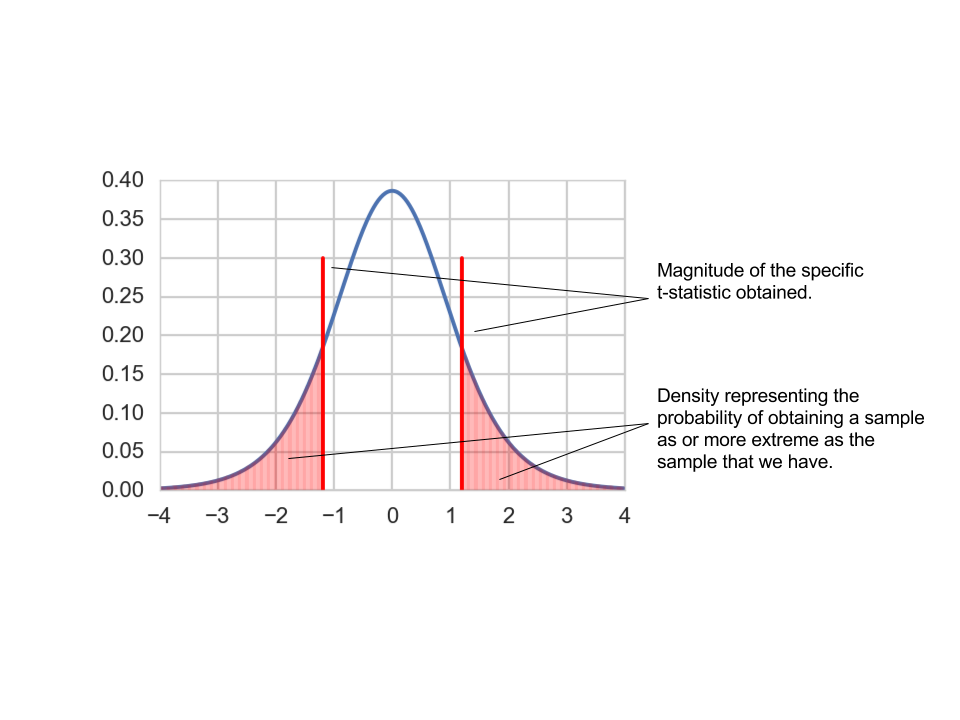
\includegraphics[width=15cm]{t_dist}
\caption{Figure showing the reference t-distribution (with 8 degrees of freedom) and the magnitude of the test statistic achieved in this example}\label{fig:t-dist}
\end{figure}

Note that as our linear model complexity increases, we may not want to test relations in isolation and moreover, despite our model assumptions, there may be some \textit{correlation} among predictor variables that affect the inferences that we make from a given model. We can then run a statistical test that accounts for multiple variables at once, this is the F-test (\ref{f-test}) derived from the \href{https://en.wikipedia.org/wiki/Analysis_of_variance}{ANOVA} test.

\newpage
\subsection{F-test}\label{f-test}
Assuming the above assumptions are met, for two nested models (i.e. consider model 1 ($M_1$) and model 2 ($M_2$) where $M_2$ contains all of the predictors of $M_1$ and more), we can test whether the additional parameters of $M_2$ form a significantly better model than those found in $M_1$.

\noindent\fbox{\begin{minipage}{\dimexpr\textwidth-2\fboxsep-2\fboxrule\relax}
\center
\textbf{Null and Alternative Hypotheses:}
\begin{align*}
H_0:&  \beta_1 = \dots = \beta_p = 0\\
H_A:& \beta_j \neq 0, \textit{for at least one value of j}
\end{align*}
\end{minipage}}

To start, we consider the $R^2$ which is the proportion of the overall variability of Y that is explained by the model $\hat{Y}$.

$$
R^2 = \frac{MSS}{TSS} = 1 - \frac{RSS}{TSS} = \frac{TSS - RSS}{TSS}
$$
with $MSS = \sum\limits_{i=1}^{N}(\hat{y}_i - \bar{y})^2$, $TSS = \sum\limits_{i=1}^{N}(y_i - \bar{y})^2$, $RSS = \sum\limits_{i=1}^{N}(y_i - \hat{y}_i)^2$

The F-test then tests if all of the $\beta_j$ coefficients are 0. Essentially, if the model explains `most' of the variance in the system, there is evidence that at \textit{least one of the predictors} must be linearly associated with the response. We are comparing the ratio of the average amount of variance that each predictor explains to the average amount of variance that is left unexplained in the model.

\begin{equation}\label{eq:f-stat}
f = \frac{\textit{Explained Variance}}{\textit{Unexplained Variance}} = \frac{(TSS - RSS)/p}{RSS/(n-p-1)}
\end{equation}

This statistic can be shown to follow a F-distribution:
\begin{align*}\label{eq:f-stat-derivation}
f &= \frac{(TSS - RSS)/p}{RSS/(n-p-1)}\\
&=  \frac{(\sum\limits_{i=1}^{N}(\frac{\hat{y}_i - \bar{y}}{\sigma})^2)/p}{(\sum\limits_{i=1}^{N}(\frac{y_i - \bar{y}}{\sigma})^2)/(n-p-1)} \sim \frac{\chi^2_{p}/p}{\chi^2_{n-p-1}/(n-p-1)} \sim F_{p, n-p-1}
\end{align*}
% The key to understanding this is that we have only dealt with a small subset of data that represents a random sample from the underlying true system. Thus, the parameters of our model have a mean and a variance associated with them. Specifically, we could notice a value for any one parameter ($\beta_j$) being $\hat{\beta_j}$. However, if the sampled standard deviation ($S$) of that parameter is much larger than $\hat{\beta_j}$, then there is no statistically robust conclusion that we can draw (i.e. our observation of $\hat{\beta_j}$ may just be a result of noise in the system and may not be due to an actual relationship). Similarly, if $S << \hat{\beta_j}$ then we can conclude, with statistical evidence, that our observation of $\hat{\beta_j}$ does not fit the null hypothesis and thus we reject this hypothesis (accepting that there is evidence for a linear relationship between that predictor and the response variable).

% So where does this test come from? The quotient of two Chi-squared random variables is said to follow an f-distribution. In our case, we are comparing the ratio of the the `Explained Variance' in the system to the `Unexplained Variance'. Recall that the definition for \textit{sample variance} is:
% $$
% s^2 = \frac{1}{n-1}\sum\limits_i(y_i - \bar{y})^2
% $$
% which follows a Chi-squared distribution. Since the `Explained Variance' and `Unexplained Variance' are themselves sample variances (we are dealing with a sample from the generative system of the data), we have a ratio of two Chi-squares and thus this statistic follows an f-distribution.
%
% Fully, we would compute the test statistic under the assumption that the Null Hypothesis is true (note the ratio of two Chi-squared distributions with their associated degrees of freedom):
% $$
% F = \frac{\textit{Explained Variance}}{\textit{Unexplained Variance}} = \frac{\frac{\sum_i (y_i - \bar{y})^2}{p}}{\frac{\sum_i (y_i - \hat{y}_i)^2}{n-p-1}} = \frac{\chi^2_{p}}{\chi^2_{n-p-1}}
% $$

\noindent\fbox{\begin{minipage}{\dimexpr\textwidth-2\fboxsep-2\fboxrule\relax}
\center
\textbf{Be careful:} Violations of the assumptions (linearity/homoskedasticity/Gaussian noise) can lead to incorrect results.
\end{minipage}}

\bibliography{section_1}
\bibliographystyle{ieeetr}
[3] Ryan Lee's class notes

[4] CS109a Lecture Notes

\end{document}
